\documentclass[sigconf,natbib=true, review=true]{acmart} %
\usepackage{graphicx} % Required for inserting images
\usepackage[show]{chato-notes}
\usepackage{amsmath}
\usepackage{algorithm}
\usepackage{subfig}
\usepackage{algpseudocode}
\usepackage{url}
\usepackage{makecell}
\usepackage{enumitem}
\usepackage{placeins}
\usepackage{multirow}

\usepackage{marginnote}
%\newcommand{\pageenlarge}[1]{\marginnote{#1}\enlargethispage{#1\baselineskip}}
\newcommand{\pageenlarge}[1]{\marginnote{}\enlargethispage{#1\baselineskip}}
%\newcommand{\pageenlarge}[1]
%\newcommand{\sasha}[1]{\textcolor{ACMred}{#1}}
%\newcommand{\sasha}[1]{\textcolor[HTML]{FF0000}{#1}}
%\newcommand{\craig}[1]{\textcolor{red}{#1}}
%\newcommand{\nt}[1]{\textcolor{blue}{#1}}

\newcommand{\sasha}[1]{\textcolor[HTML]{000000}{#1}}
\newcommand{\rsasha}[1]{\textcolor[HTML]{FF0000}{#1}}
\newcommand{\craig}[1]{\textcolor{black}{#1}}
\newcommand{\nt}[1]{\textcolor{black}{#1}}

\newcommand{\argmax}{\operatornamewithlimits{\sf argmax}}



%\title{Pruning sub-item representations for large-catalogue recommender models}
\title{Efficient Inference of Sub-Id based models with Millions of Items}
\copyrightyear{2024} 
\acmYear{2024} 

\begin{CCSXML}
<ccs2012>
   <concept>
       <concept_id>10002951.10003317</concept_id>
       <concept_desc>Information systems~Information retrieval</concept_desc>
       <concept_significance>500</concept_significance>
       </concept>
 </ccs2012>
\end{CCSXML}

\ccsdesc[500]{Information systems~Information retrieval}

%
% Keywords. The author(s) should pick words that accurately describe
% the work being presented. Separate the keywords with commas.
\keywords{Recommender Systems, Inferenece}


\setcopyright{acmlicensed}\acmConference[SIGIR '24]{Fourty Seventh International ACM SIGIR Conference on Research and Development in Information Retrieva}{July 14--18, 2024}{Washington D.C., USA}
\acmBooktitle{Fourty Seventh International ACM SIGIR Conference on Research and Development in Information Retrieval (SIGIR '24), July 14--18, 2024, Washington D.C., USA}


\author{Anonymous Author(s)}
\affiliation{%
  \institution{Organisation} \country{A Country}}
\email{email@example.com}



% \author{Aleksandr V. Petrov}
% \affiliation{%
%   \institution{University of Glasgow} \country{United Kingdom}}

% \email{a.petrov.1@research.gla.ac.uk}

% \author{Craig Macdonald}
% \affiliation{%
%   \institution{University of Glasgow} \country{United Kingdom}}
% \email{craig.macdonald@glasgow.ac.uk}



% \author{Nicola Tonellotto}
% \affiliation{%
%   \institution{University of Pisa} \country{Italy}}
% \email{nicola.tonellotto@unipi.it}
\begin{document}

\begin{abstract}
Transformer-based recommender systems, such as BERT4Rec or SASRec, achieve state-of-the-art results in sequential recommendation. However, these models are still rarely used in the real-world recommendation. The major challenge of adapting these models is the catalogue size: in production, it is common to have millions of items in the catalogue, while scaling transformers beyond a few thousand items is problematic due to large GPU memory requirements, inefficient training and slow inference. Several recent papers addressed inefficient training and large memory requirements, but slow inference with large catalogues remains problematic. In particular, RecJPQ is a state-of-the-art method of reducing the model's memory consumption; RecJPQ achieves compression by decomposing item IDs into a small number of shared sub-item IDs. Despite reporting the reduction of memory consumption by a factor of up to 50x, the original RecJPQ paper did not report any inference efficiency improvements over the baseline transformer-based models. However, several earlier works based on similar ideas suggest that fast inference is possible when using sub-id decomposition. In this paper, we analyse the source of discrepancy between RecJPQ and similar work and find that the original RecJPQ code does not utilise inference optimisation techniques, such as execution graph compilation. We find that by utilising PQTopK, an efficient scoring algorithm, combined with optimisation techniques, such as graph compilation and avoiding converting data types (e.g. converting tensors to numpy arrays), we can speed up RecJPQ inference by \inote{XXX} times on a large-scale Gowalla dataset. Using simulated data, we show that PQTopK remains efficient with catalogues up to \inote{YYY million items}, removing one of the last obstacles for using transformer-based models in production.
\end{abstract}

\maketitle

\section{Background} \label{ssec:recsys:preliminarilies}
\subsection{Transformers for Large-catalogue Sequential Recommendation}\label{sec:rec}

\looseness -1 Usually, sequential recommendation is cast as the \emph{next item prediction} task. Formally, given a chronologically ordered sequence of user-item interactions $\left\{i_1, i_2, i_3 ... i_n\right\}$, \nt{also known as their \textit{interactions history},} the goal of a recommender system is to predict the next item in the sequence, $i_{n+1}$ from the \emph{item catalogue} (the set of all possible items) $I$. The total number of items $|I|$ is the \emph{catalogue size}.

% \inote{cannot parse this sentence} \inote{Nic: the following sentence fits more in introduction or related works IMO.}
Sequential recommendation bears a resemblance to the natural language processing task of \emph{next token prediction}, as addressed by language models, such as GPT-2~\cite{gpt2}.
%In the natural language processing domain, a similar task is the \emph{next token prediction} task, which is one of the most common tasks in generative language models, such as GPT-2~\cite{gpt2}. 
Hence, researchers have adapted language models to the recommendation task by replacing token IDs (in language models) with item IDs (in recommendation models). In particular, Transformer~\cite{Transformer}-based models, such as SASRec~\cite{SASRec} (based on the Transformer Decoder architecture, similar to GPT-2~\cite{gpt2})  and BERT4Rec~\cite{BERT4Rec} (based on Transformer Encoder, similar to BERT) have demonstrated state-of-the-art results for sequential recommendation~\cite{Bert4RecRepro}. 


Typically, to generate recommendations given a history of interactions $h = \left\{i_1, i_2, i_3 ... i_n\right\}$, Transformer-based models first generate a sequence embedding $\phi \in \mathbb{R}^d$, where $d$ is the embedding dimensionality, using the Transformer model, such that $\phi =  \textsf{Transformer}(h)$\footnote{In document retrieval parlance, this would be a query embedding.}.
% \begin{align}
% \phi =  \textsf{Transformer}(h)
% \end{align}
The scores for all items, $r = (r_1, \ldots, r_{|I|}) \in \mathbb{R}^{|I|}$, are then computed by multiplying the matrix of item embeddings $W \in \mathbb{R}^{|I|\times d}$, which is usually shared with the embeddings layer of the Transformer model, by the sequence embedding $\phi$\footnote{This also generalises to models that have item biases (e.g.\ BERT4Rec), if we assume that the first dimension of sequence embedding equals 1 and the first dimension of item embedding contains item bias.}:
\begin{align}
r = W\phi\label{eq:scores}
\end{align}

Finally, the model generates recommendations by selecting for $r$ the top $K$ items with the highest scores.%:
%\begin{align}
%    \text{Recommendations} = \textsf{TopK}(R, k)
%k\argmax_{i \in I} (r_i)
%\end{align}\inote{I dont follow this eqn}

Despite their effectiveness, training Transformer-based models with large item catalogues is a challenging task, as these models typically have to be trained for long time~\cite{Bert4RecRepro} and require appropriate selection of training objective~\cite{petrovRSSEffectiveEfficient2023}, negative sampling strategy and loss function~\cite{petrovGSASRecReducingOverconfidence2023,klenitskiyTurningDrossGold2023}.
%
Transformer-based models with large catalogues also require a lot of memory to store the item embeddings $W$. This problem has recently been addressed by Product Quantiantisation, which we describe in the next section. 
%
Finally, another problem with transformer-based models with large catalogues is their slow inference with large catalogues. Indeed, computing all item scores using Equation~\eqref{eq:scores} may be prohibitively expensive when the item catalogue is large: it requires $|I|\times d$ scalar multiplications and additions, and, as we noted in Section~\ref{sec:intro},  in real-world recommender systems, the catalogue size $|I|$ may reach hundreds of millions of items, making exhaustive computation using Equation~\eqref{eq:scores} impractical. Moreover, typically large-catalogue recommender systems have a large number of users as well; therefore, the model has to be used for inference very frequently, and, ideally, using only low-cost hardware, i.e., without using GPU acceleration. Therefore, real-life recommender systems rarely exhaustively score all items for all users and instead apply unsafe heuristics (i.e.\ heuristics that do not provide theoretical guarantees that all high-scored items will be returned, such as two-stage ranking). 
 
 %\pageenlarge{1}
\section{Sub-Id based recommendation}\label{ssec:recjpq}


\begin{figure}[tb]\hspace{-3mm}
    \vspace{-0.5\baselineskip}
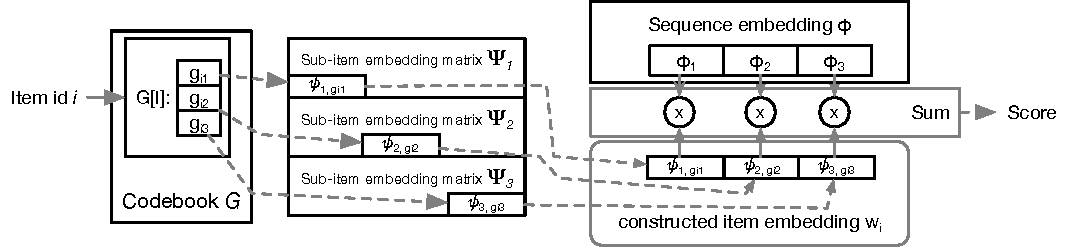
\includegraphics[width=0.5\textwidth]{figures/pq_scoring_graffle.pdf}%\vspace{-.75\baselineskip}
    \caption{Reconstruction of item embeddings \sasha{and computing item scores} using Product Quantisation \sasha{with $m=3$ splits.} }\vspace{-.75\baselineskip}
    \label{fig:embedding_reconstruction}
\end{figure}


As we noted above, with large item catalogues, the item embedding matrix $W$ requires too much memory to store. Indeed, when the catalogue size reaches several million items, the item embedding matrix becomes too large to fit in a GPU's memory~\cite{petrovRecJPQTrainingLargeCatalogue2024}. To reduce its memory footprint, several recent recommendation models adopted Product Quantisation (PQ)~\cite{jegouProductQuantizationNearest2011} -- a well-studied method for vector compression. PQ is a generic method that can be applied to any \nt{set of vectors}; however, in this section, we \nt{describe} PQ as applied to item embedding. 

\looseness -1 To compress the item embedding matrix $W$, PQ associates each item id to a list of {\em sub-ids}, akin to language models breaking down words into sub-word tokens. PQ reconstructs an item's embedding by combining the sub-id embeddings assigned to it. These sub-ids are organised into {\em splits}, with each item having precisely one sub-id from each split\footnote{We use the terminology from~\cite{petrovRecJPQTrainingLargeCatalogue2024}. In the PQ literature, another popular term for sub-id embeddings is \emph{centroids}, and another popular term for splits is \emph{sub-spaces}.}. More formally, PQ first builds a \emph{codebook} $G\in\mathbb{N}^{|I|\times m}$ that maps an item id $i$ to its associated $m$ sub-ids:
\begin{align}
    G[i] \rightarrow \left\{g_{i1}, g_{i2}, ..., g_{im}\right\} \label{eq:sub_ids_map}
\end{align}
where $g_{ij}$ is the $j$-th sub-id associated with item $i$ and $m$ is the number of splits. To achieve compression compared to storing a full item embedding matrix, $m$ is typically chosen much smaller compared to full embeddings dimensionality: $m \ll d$.
The exact algorithm for associating ids with sub-ids is specific to different implementations of PQ. For example, the original PQ implementation uses variations of K-Means clustering, Differentiable Product Quantisation proposes a method to learn the mapping~\cite{chenDifferentiableProductQuantization2020} as part of overall model training, and RecJPQ~\cite{petrovRecJPQTrainingLargeCatalogue2024} derives the codes from a truncated SVD decomposition of the user-item interactions matrix. 

%\pageenlarge{1}

For each split $k=1,\ldots,m$, PQ stores a sub-item embedding matrix $\Psi_k \in \mathbb{R}^{b\times\frac{d}{m}}$, where $b$ is the number of distinct sub-ids in each split. The $j$-th row of $\Psi_k$ denotes the sub-item embedding $\psi_{k,j} \in \mathbb{R}^{\frac{d}{m}}$ associated with the $j$-th sub-id, in the $k$-th split.
Then, PQ reconstructs the item embedding $w_i$ as a concatenation of the associated sub-id embedding: 
\begin{align}
    w_i =  \psi_{1,g_{i1}} \mathbin\Vert \psi_{2,g_{i2}}  \mathbin\Vert ... \mathbin\Vert  \psi_{m,g_{im}} \label{eq:pq:item_embedding}
\end{align}

Finally, an item score is computed as the dot product of the  sequence embedding and the constructed item embedding: 
\begin{align}
    r_i = w_i \cdot \phi\label{eq:dot_product}
\end{align}

\section{PQTopK}
\looseness -1 A straightforward use of Equation~\eqref{eq:dot_product} for item scoring in PQ-based recommendation models does not lead to any computational efficiency improvements compared to models where all item embeddings are stored explicitly.
However, PQ offers a more efficient scoring algorithm. To achieve more efficient scoring, PQ  first splits the sequence embedding $\phi \in \mathbb{R}^{d}$ into $m$ sub-embeddings $\left\{\phi_1, \phi_2 ... \phi_m\right\}$, with $\phi_{k} \in \mathbb{R}^{\frac{d}{m}}$ for $k=1, \ldots,m$, such that $\phi = \phi_1  \mathbin\Vert \phi_2  \mathbin\Vert ... \mathbin\Vert  \phi_m$.
By substituting Equation~\eqref{eq:pq:item_embedding} and the similarly decomposed sequence embedding $\phi$ into Equation~\eqref{eq:dot_product}, we can compute the final item score for item $i$ as the sum of sub-embedding dot-products: 
\begin{align}
  %r_i = w_i \cdot \phi &= (\psi_{1,g_{i1}} \mathbin\Vert \psi_{2,g_{i2}}  \mathbin\Vert ... \mathbin\Vert  \psi_{m,g_{im}}) \cdot (\phi_1  \mathbin\Vert \phi_2  \mathbin\Vert ... \mathbin\Vert  \phi_m) \nonumber \\
  %&= \sum_{k=1}^m \psi_{k,g_{ik}} \cdot \phi_k
   r_i = w_i \cdot \phi &= (\psi_{1,g_{i1}} \mathbin\Vert ... \mathbin\Vert  \psi_{m,g_{im}}) \cdot (\phi_1  \mathbin\Vert ... \mathbin\Vert  \phi_m) = \sum_{k=1}^m \psi_{k,g_{ik}} \cdot \phi_k \nonumber
\end{align}

Let $S \in \mathbb{R}^{m \times b}$ denote the \emph{sub-id score matrix}, which consists of \emph{sub-id scores} $s_{k,j}$, defined as dot products of the sub-item embedding $\psi_{k,j}$ and the sequence sub-embeddings $\phi_k$:
\begin{align}
s_{k,j} = \psi_{k,j} \cdot \phi_k\label{eq:sub_item_scores}
\end{align}

The final score of item $i$ is then can be computed as the sum of the scores of its associated sub-ids:
\begin{align}
   r_{i} = \sum_{k=1}^m s_{k,g_{ik}} \label{eq:sum_sub_scores}
\end{align}

The number of splits $m$ and the number of sub-ids per spit $b$ are usually  chosen to be relatively small, 
so that the total number of sub-id scores is much less compared to the size of the catalogue, e.g., $m\times b \ll |I|$. 
%\begin{align}
%m\times b \ll |I| \label{eq:sub_items_scores_size}
%\end{align}
%
Therefore,  we can pre-compute matrix $S$ \sasha{for a given sequence embedding} once and then reuse these scores for all items. This leads to efficiency gains compared to matrix multiplication, as scoring each item now only requires $m \ll d$ additions instead of $d$ multiplications and $d$ additions per item (Equation~\eqref{eq:scores}). The time for pre-computing sub-item scores matrix $S$ does not depend on the catalogue size $|I|$, and %according to Equation~\eqref{eq:sub_items_scores_size},
we can assume that it is negligible compared to exhaustive scoring of all items. 

%\pageenlarge{1} 
In the paper, we refer to the summation-based approach as \textit{PQTopK}; Algorithm~\ref{alg:top_k} illustrates the PQTopK in pseudo-code. \rsasha{PQTopK} allows selecting top $K$ items not only from all items but from a specific subset of items.



\begin{algorithm}[h]
\small
\caption{PQTopK($G$, $S$, $K$, $V$). This is a simple summation-based scoring algorithm used by the RecJPQ method.}\label{alg:top_k}
\begin{algorithmic}[1]
   \Require $G$ is the codebook (mapping: item id $\rightarrow$ sub-item ids), Eq.~\eqref{eq:sub_ids_map}
   \Require $S$ is the matrix of pre-computed sub-item scores, indexed by split and sub-item, Eq.~\eqref{eq:sub_item_scores}

   \Require $K$ is the number of results to return
%   %\Require $m$ is the number of splits
   \Require $V \subseteq I$ are the items to score; all items ($V = I$)  if not given 
   
   \State $scores \gets$ empty array of scores for all items in $V$, initialised to 0
   \For{$item\_id \in V$}
        % \State $accum \gets 0$
        % \For{$split\_id, subitem\_id \in \textsf{enumerate}(G[item\_id]$)}
        %     \State $accum \gets accum + S[split\_id, subitem\_id]$
        % \EndFor
        \State $score[item\_id] \gets \sum_{k=1}^{m} S[k,G[item\_id,k]] $ \Comment{Eq.~\eqref{eq:sum_sub_scores}}
   \EndFor
   \State \Return TopK($score$, $K$) \Comment{Returns a list of $\langle$ItemId, Score$\rangle$ pairs} 
\end{algorithmic}
\end{algorithm}
\begin{table}
\resizebox{\linewidth}{!}{
    % Please add the following required packages to your document preamble:
% \usepackage{multirow}
    \begin{tabular}{|l|l|cccccc|}
    \hline
                               &                     & \multicolumn{3}{c|}{Dataset: Booking}                                                                                                                                                                                                  & \multicolumn{3}{c|}{Dataset: Gowalla}                                                                                                                                                                            \\ \hline
                   & Scoring method      & \begin{tabular}[c]{@{}c@{}}mRT\\ (Scoring)\end{tabular} & \begin{tabular}[c]{@{}c@{}}mRT\\ (Total)\end{tabular} & \multicolumn{1}{l|}{\begin{tabular}[c]{@{}l@{}}Backbone\\ measures\end{tabular}}                                    & \begin{tabular}[c]{@{}c@{}}mRT\\ (Scoring)\end{tabular} & \begin{tabular}[c]{@{}c@{}}mRT\\ (Total)\end{tabular} & \begin{tabular}[c]{@{}l@{}}Backbone\\ measures\end{tabular}                                    \\ \hline
    \multirow{4}{*}{\rotatebox{90}{gBERT4Rec}} & Transformer Default & 6.22                                                    & 43.37                                                 & \multicolumn{1}{l|}{\multirow{4}{*}{\begin{tabular}[c]{@{}c@{}}NDCG@10: \\ 0.3281, \\ Model mRT: \\37.16\end{tabular}}}  & 133.40                                                  & 171.04                                                & \multirow{4}{*}{\begin{tabular}[c]{@{}c@{}}NDCG@10: \\ 0.1684\\  Model mRT: \\ 37.52\end{tabular}} \\
                               & RecJPQ-Original     & 3.9                                                     & 41.08                                                 & \multicolumn{1}{l|}{}                                                                                               & 33.87                                                   & 71.42                                                 &                                                                                                \\
                               & RecJPQ-Optimised    & 5.33                                                    & 42.46                                                 & \multicolumn{1}{l|}{}                                                                                               & 23.08                                                   & 60.66                                                 &                                                                                                \\
                               & PQ-TopK             & \textbf{3.09}                                           & \textbf{40.23}                                        & \multicolumn{1}{l|}{}                                                                                               & \textbf{13.79}                                          & \textbf{51.33}                                        &                                                                                                \\ \hline
    \multirow{4}{*}{\rotatebox{90}{SASRec}}    & Transformer Default & 6.27                                                    & 30.03                                                 & \multicolumn{1}{l|}{\multirow{4}{*}{\begin{tabular}[c]{@{}c@{}}NDCG@10:\\ 0.1886\\  Model mRT:\\ 23.75\end{tabular}}} & 131.35                                                  & 156.07                                                & \multirow{4}{*}{\begin{tabular}[c]{@{}c@{}}NDCG@10: \\ 0.1209\\  Model mRT: \\ 24.67\end{tabular}} \\
                               & RecJPQ-Original     & 3.77                                                    & 27.53                                                 & \multicolumn{1}{l|}{}                                                                                               & 29.65                                                   & 54.32                                                 &                                                                                                \\
                               & RecJPQ-Optimised    & 5.15                                                    & 28.93                                                 & \multicolumn{1}{l|}{}                                                                                               & 19.85                                                   & 44.55                                                 &                                                                                                \\
                               & PQ-TopK             & \textbf{2.93}                                           & \textbf{26.69}                                        & \multicolumn{1}{l|}{}                                                                                               & \textbf{10.03}                                          & \textbf{34.72}                                        &                                                                                                \\ \hline
    \end{tabular}
}
\end{table}

\bibliographystyle{ACM-Reference-Format}
\balance
\bibliography{references}

\end{document}
